\chapter{Curved Space and the Geometry of Cosmology}

These notes follow Leonard Susskind's third cosmology lecture closely. The preserved board frames from LazyingArt LLC and Video2Book are used only as documentary support for the visible equations and sketches; the transcript remains the primary guide to the order of ideas. The lecture opens by undoing a convenience. We have been assuming flat space because it is observationally a good approximation, but flatness is not a principle. Before one can speak responsibly about cosmology, one must ask what homogeneous space could be if it were not flat, and only then return to the dynamics of expansion.

\section{Why Cosmology Must Reopen Geometry}

We begin with a warning that is characteristic of the whole lecture. Observation tells us that space is very flat on the scales we can probe, but that is not the same as saying that space \emph{must} be flat. It may be flat, positively curved, or negatively curved. The right response is not to pick one case dogmatically, but to investigate the alternatives.

The lecture immediately narrows the possibilities by keeping one assumption while dropping another. We set aside flatness, but we continue---for the moment---to assume homogeneity and isotropy. Homogeneity means that every observer sees the same local geometry. That one sentence already excludes a great many curved spaces. A paraboloid is curved, but not everywhere in the same way. An ellipsoid is curved, but the poles and the waist are geometrically different. A bumpy surface is curved, but the bumps themselves betray special places. None of these is suitable as a cosmological model if one wants a geometry that looks the same from every point.

So the lecture does not ask, ``What curved spaces can we draw?'' It asks instead, ``What curved spaces are homogeneous?'' That is the question that forces us toward the very small family of constant-curvature geometries: flat space, spherical space, and hyperbolic space. Before we distinguish them, however, we need the real language of geometry, namely the metric.

\section{Metrics, Polar Coordinates, and the Unit Circle}

A geometry is specified by its metric: the squared distance between neighboring points. In flat three-dimensional Euclidean space the opening example is the familiar line element
\begin{equation}
ds^2 = dx^2 + dy^2 + dz^2.
\end{equation}

\begin{figure}[htbp]
\centering

\includegraphics[width=0.74\textwidth]{lecture_03_figure_02.png}
\caption{Flat-space metric in Cartesian coordinates, as written on the board.}
\end{figure}

In two dimensions the same geometry would be
\begin{equation}
ds^2 = dx^2 + dy^2.
\end{equation}
If we add a third Cartesian direction, we add \(dz^2\), and that is all. The point is not the formula itself. The point is that once the metric is known, the geometry is known.

Susskind then changes coordinates, not for algebraic amusement, but because cosmology is naturally observer-centered. We look out into the sky by angles. In a two-dimensional world our visual field would literally be a field of angles, so polar coordinates are the natural language. Introducing a radial coordinate \(r\) and an angular coordinate \(\theta\), the metric becomes
\begin{equation}
ds^2 = dr^2 + r^2 d\theta^2.
\end{equation}
Since the lecture immediately promotes the angular part into a reusable symbol, we standardize the notation as
\begin{equation}
d\Omega_1^2 = d\theta^2,
\qquad\text{so that}\qquad
ds^2 = dr^2 + r^2 d\Omega_1^2.
\end{equation}
On the board the subscript is not legible, but the transcript makes clear that the intended object is the metric of the unit \(1\)-sphere.

\begin{figure}[htbp]
\centering

\includegraphics[width=0.74\textwidth]{lecture_03_figure_03.png}
\caption{Flat space written in polar form; the board shows \(d\Omega^2\), which the lecture identifies with the metric of the unit circle.}
\end{figure}

\begin{figure}[htbp]
\centering
\begin{tikzpicture}[scale=1.2]
\draw[->] (-1.2,0)--(1.7,0);
\draw[->] (0,-1.2)--(0,1.7);
\draw[thick] (0,0)--(1.25,1.05);
\draw (0.72,0.65) node[above] {$r$};
\draw (0.55,0) arc (0:40:0.55);
\draw (0.78,0.2) node {$\theta$};
\end{tikzpicture}
\caption{A clean redraw of the polar-coordinate sketch that accompanies the metric \(ds^2 = dr^2 + r^2 d\Omega_1^2\).}
\end{figure}

The factor \(r^2\) carries the geometrical content. If two points differ only in angle, then the arc length between them grows linearly with \(r\), and the squared distance grows like \(r^2\). This is exactly the statement that circles centered on us get larger and larger in proportion to their radius.

\subsection{Question \& Answer}

Why does \(d\theta^2\) count as the metric of a circle?

Because on a unit circle the only intrinsic coordinate is the angular coordinate itself. Two neighboring points separated by \(d\theta\) differ by an arc length \(d\theta\), so the squared distance along the circle is \(d\theta^2\). In that sense \(d\theta^2\) is already a metric before it is inserted into the polar metric of the plane.

This is also the moment when the lecture insists on the difference between intrinsic and extrinsic thinking. If we insist on embedding the unit circle in a plane, we can write it as
\begin{equation}
x^2 + y^2 = 1.
\end{equation}
But that is only one way of drawing it. Intrinsically, the circle is simply a one-dimensional space that closes on itself and has total length \(2\pi\). The same metric \(d\theta^2\) would describe a deformed loop, provided equal increments of \(\theta\) still correspond to equal distances along it. The drawing may cease to look round, but the metric need not change.

\begin{figure}[htbp]
\centering

\includegraphics[width=0.64\textwidth]{lecture_03_figure_04.png}
\caption{A round unit circle and a deformed but metrically equivalent closed loop.}
\end{figure}

\begin{figure}[htbp]
\centering
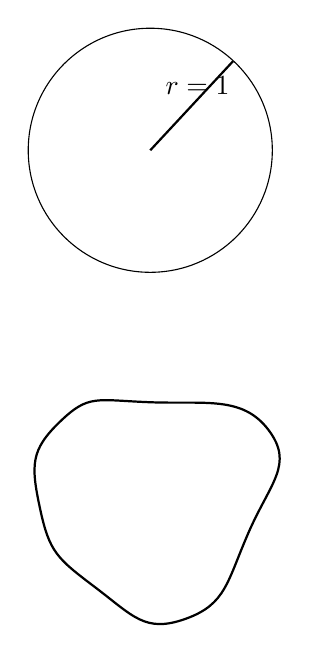
\begin{tikzpicture}[scale=1.0]
\draw (0,0) circle (1.55);
\draw[thick] (0,0)--(1.05,1.13);
\draw (0.6,0.82) node {$r=1$};

\begin{scope}[yshift=-4.4cm]
\draw[thick]
plot[smooth cycle, tension=0.95] coordinates
{(0,1.2) (1.5,0.85) (1.25,-0.45) (0.45,-1.55) (-0.7,-1.15) (-1.4,-0.15) (-1.15,0.95)};
\end{scope}
\end{tikzpicture}
\caption{A schematic redraw of the lecture's point: ``circle'' is an intrinsic metric notion, not merely a Euclidean appearance.}
\end{figure}

Returning now to the plane, each concentric circle around us has its own radius \(r\), and therefore each one contributes \(r^2 d\Omega_1^2\) to the angular part of the metric. That is why the flat plane can be thought of as a nested family of circles whose size grows linearly with distance.

\section{Positive Curvature: The 2-Sphere and the 3-Sphere}

The next step is the crucial one. A sphere is curved, but unlike a paraboloid or an ellipsoid it is still homogeneous. Every point on a sphere is the same as every other point. So we now ask: what replaces the family of circles of radius \(r\) when the plane is replaced by a sphere?

Here the lecture makes a deliberate change in viewpoint. We imagine ourselves as astronomers living on a \(2\)-sphere and looking outward from our own position. Near us we see a small surrounding circle. Farther away we see a larger one. Farther still, a larger one again. But now the behavior is different from the plane: the circles do not continue to grow forever. Their growth slows, reaches a maximum, and then reverses. The key point is that this is a statement about \emph{distance}, not about \emph{time}. We are still doing static geometry.

At this stage the notation must be reset. On the unit \(2\)-sphere we use \(r\) to denote the angular distance from our chosen origin. Thus
\[
0 \le r \le \pi.
\]
At \(r=0\) we are at our own point. At \(r=\pi/2\) we are at the equator. At \(r=\pi\) we have reached the antipode. On the unit sphere the circles surrounding us have radius \(\sin r\), so the flat factor \(r^2\) is replaced by \(\sin^2 r\). The canonical metric is therefore
\begin{equation}
d\Omega_2^2 = dr^2 + \sin^2 r\, d\Omega_1^2
           = dr^2 + \sin^2 r\, d\theta^2.
\end{equation}
The board line in the lecture is only partially visible, but the spoken derivation makes the intended replacement unambiguous: the angular factor is \(\sin^2 r\), not \(r^2\).

\begin{figure}[htbp]
\centering

\includegraphics[width=0.82\textwidth]{lecture_03_figure_05.png}
\caption{The lecture's transition board from flat radial geometry to spherical radial geometry. The lower spherical line is only partially visible in the frame, but the transcript fixes the intended replacement \(r^2 \mapsto \sin^2 r\).}
\end{figure}

\begin{figure}[htbp]
\centering
\begin{tikzpicture}[scale=0.92]
\begin{scope}[xshift=-4.0cm]
\draw[->] (-1.7,0)--(1.9,0);
\draw[->] (0,-1.7)--(0,1.9);
\draw (0,0) circle (0.45);
\draw (0,0) circle (0.9);
\draw (0,0) circle (1.35);
\draw[thick] (0,0)--(1.45,1.2);
\draw (0.55,0.18) arc (18:40:0.62);
\draw (0.92,0.42) node {$\theta$};
\end{scope}

\begin{scope}[xshift=4.0cm]
\draw (0,0) circle (2.0);
\fill (0,-2.0) circle (1.5pt);
\fill (2.0,0) circle (1.5pt);
\fill (0,2.0) circle (1.5pt);
\draw[thick] (0,-2.0) arc (-90:90:2.0);
\draw (0,-2.35) node {$r=0$};
\draw (2.75,0) node {$r=\pi/2$};
\draw (0,2.35) node {$r=\pi$};
\end{scope}
\end{tikzpicture}
\caption{A clean reconstruction of the lecture's two pictures: flat space as nested circles, and the sphere as a family of circles that grow, reach a maximum, and then shrink back to zero.}
\end{figure}

The notation continues recursively. Once the metric of the \(2\)-sphere has been built, it becomes the angular part of the \(3\)-sphere. We also write flat three-dimensional space in the same radial language:
\begin{align}
ds_{\text{flat},3}^2 &= dr^2 + r^2 d\Omega_2^2,\\
d\Omega_3^2 &= dr^2 + \sin^2 r\, d\Omega_2^2.
\end{align}
This is exactly the same pattern one dimension up. Around us sit nested \(2\)-spheres rather than nested circles. At first they grow, then they reach a largest \(2\)-sphere, and then they shrink again to a point.

For visualization only, one may embed the unit \(2\)-sphere in Euclidean three-space as
\begin{equation}
x^2+y^2+z^2=1.
\end{equation}
Likewise, one may think of the unit circle as \(x^2+y^2=1\). But the lecture repeatedly warns us not to confuse these embeddings with the intrinsic geometry. The \(3\)-sphere is not the boundary of an ordinary ball in our familiar three-dimensional space. It is itself a three-dimensional space.

\subsection{Question \& Answer}

Is the observer at the center of the sphere, or only at the center of the chosen coordinates?

Only at the center of the chosen coordinates. On the sphere there is no distinguished center \emph{in the geometry itself}. We place ourselves at \(r=0\) because any point may be used as the origin from which distances are measured. That is exactly what homogeneity means. The same warning applies even more strongly to the \(3\)-sphere: the nested family of \(2\)-spheres is a family of shells \emph{around us}, not evidence for a genuine central point of the universe.

\section{How an Astronomer Would Detect a Sphere}

Once the metric is written down, the lecture turns immediately to observation. How would an astronomer tell whether she lived in flat space or on a sphere?

Take a standard object of true diameter \(d\). First consider flat space. If the object lies at fixed radial distance \(r\), then along its transverse extent we have \(dr=0\), so the metric reduces to
\begin{equation}
d^2 = r^2 d\theta^2.
\end{equation}
Thus
\begin{equation}
d\theta = \frac{d}{r}.
\end{equation}
This is the usual inverse-distance law for angular size.

Now repeat the same calculation on the sphere. The relevant transverse part of the metric is no longer \(r^2 d\theta^2\), but \(\sin^2 r\, d\theta^2\). Therefore
\begin{equation}
d^2 = \sin^2 r\, d\theta^2,
\qquad\text{so}\qquad
d\theta = \frac{d}{\sin r}.
\end{equation}
That single change carries the whole observational difference. Since \(\sin r < r\) for \(0<r<\pi\), the same galaxy at the same measured distance would look larger on a sphere than in flat space. More sharply still, beyond \(r=\pi/2\) the factor \(\sin r\) begins to decrease, so the apparent size turns around: very distant objects begin to look larger again. At the antipode, where \(r=\pi\) and \(\sin r\) returns to zero, the extreme idealization would be that an object there fills the sky.

This is not merely a formal game. The lecture emphasizes that a curvature measurement from the cosmic microwave background works in the same broad way: one identifies a standard physical scale, measures the angle it subtends, and compares that to the geometry.

A second observational test is counting. Flat space keeps opening up: shells at larger \(r\) contain more room and therefore more galaxies. On a sphere the shells first open, then close again. Near the largest possible distance there is hardly any shell left, and the number of galaxies at that distance is correspondingly small. So spherical geometry predicts two linked effects: objects look too large, and far-away shells contain too few objects.

\subsection{Question \& Answer}

How could one tell that \(r\) is approaching \(\pi\) rather than simply becoming very large?

Because here \(r\) is not an ordinary unbounded radial coordinate. It is an angular-distance coordinate on the \emph{unit} sphere. Its range is finite:
\[
0 \le r \le \pi.
\]
So ``large \(r\)'' on a sphere means ``close to the antipode,'' not ``arbitrarily far away.'' If the sphere had radius \(a\) instead of \(1\), the same story would hold after an overall rescaling, but the finite range in the unit variable would remain.

\section{Stereographic Pictures and Hyperbolic Space}

Before entering hyperbolic space, the lecture introduces a new visual habit: stereographic projection. One rests a sphere on a plane tangent at the south pole, then projects each point of the sphere to the plane by drawing the straight line from the north pole through that point. The north pole itself goes to infinity. Nearby figures are not deformed very much, but figures nearer the north pole become larger and larger on the plane.

\begin{figure}[htbp]
\centering
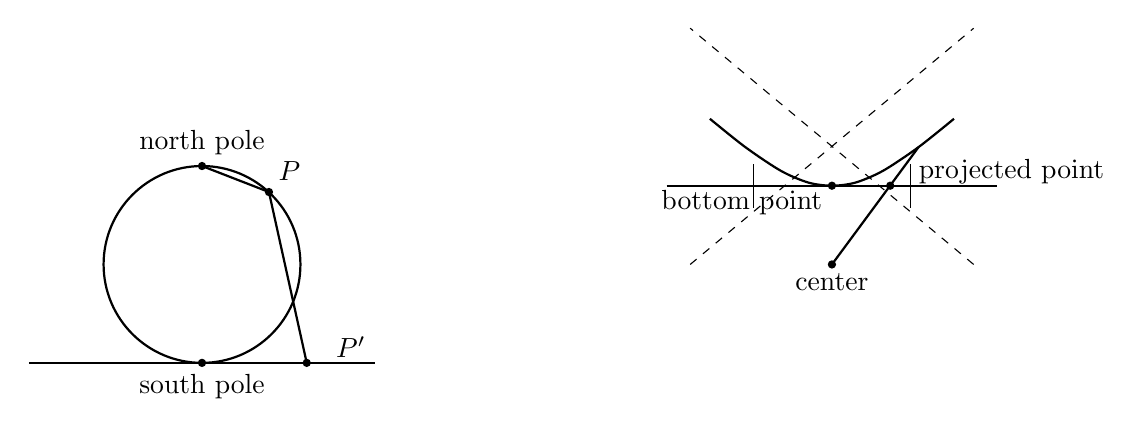
\begin{tikzpicture}[scale=1.0]
\begin{scope}[xshift=-4.0cm]
\draw[thick] (-2.2,-1.25)--(2.2,-1.25);
\draw[thick] (0,0) circle (1.25);
\fill (0,1.25) circle (1.5pt);
\fill (0,-1.25) circle (1.5pt);
\draw (0,1.55) node {north pole};
\draw (0,-1.55) node {south pole};

\fill (0.85,0.92) circle (1.5pt);
\draw (0.85,1.18) node[right] {$P$};
\draw[thick] (0,1.25)--(0.85,0.92)--(1.33,-1.25);
\fill (1.33,-1.25) circle (1.5pt);
\draw (1.58,-1.05) node[right] {$P'$};
\end{scope}

\begin{scope}[xshift=4.0cm]
\draw[thick] (-2.1,1)--(2.1,1);
\draw[dashed] (-1.8,0)--(1.8,3.0);
\draw[dashed] (1.8,0)--(-1.8,3.0);
\draw[thick]
plot[smooth] coordinates
{(-1.55,1.85) (-1.1,1.49) (-0.65,1.19) (-0.3,1.04) (0,1.0) (0.3,1.04) (0.65,1.19) (1.1,1.49) (1.55,1.85)};
\fill (0,0) circle (1.5pt);
\fill (0,1) circle (1.5pt);
\draw (0,-0.22) node {center};
\draw (0,0.78) node[left] {bottom point};
\draw[thick] (0,0)--(1.1,1.49);
\fill (0.74,1) circle (1.5pt);
\draw (0.98,1.18) node[right] {projected point};
\draw (-1,0.72) -- (-1,1.28);
\draw (1,0.72) -- (1,1.28);
\end{scope}
\end{tikzpicture}
\caption{Cross-sectional sketches of the two projection ideas used in the lecture: stereographic projection of the sphere onto a plane, and the analogous projection of the hyperboloid onto the finite disk (shown here in cross-section as a finite interval).}
\end{figure}

The sphere remains homogeneous despite this distortion, because the distortion belongs to the projection, not to the sphere. Equal intrinsic circles on the sphere project to circles of different apparent sizes on the plane.

Now the lecture introduces the third homogeneous geometry. In two dimensions its metric is
\begin{equation}
dh_2^2 = dr^2 + \sinh^2 r\, d\Omega_1^2,
\end{equation}
and in three dimensions,
\begin{equation}
dh_3^2 = dr^2 + \sinh^2 r\, d\Omega_2^2.
\end{equation}
Here \(r\) is again reset: it is now the radial coordinate of hyperbolic space, and it runs from \(0\) to \(\infty\). The shell factor is \(\sinh r\), not \(r\) and not \(\sin r\).

To explain why this matters, Susskind pauses over the exponential form
\begin{equation}
\sin r = \frac{e^{ir}-e^{-ir}}{2i},
\qquad
\sinh r = \frac{e^{r}-e^{-r}}{2}.
\end{equation}
For large \(r\), the \(\sinh r\) term is dominated by \(e^r/2\). So the shells around us in hyperbolic space grow exponentially. This flips all the spherical observational statements around. A fixed-size galaxy at fixed \(r\) satisfies
\begin{equation}
d^2 = \sinh^2 r\, d\theta^2,
\qquad\text{so}\qquad
d\theta = \frac{d}{\sinh r}.
\end{equation}
For \(r\gg 1\),
\begin{equation}
d\theta \sim 2d\, e^{-r}.
\end{equation}
Thus distant objects look anomalously small in hyperbolic space, not anomalously large. At the same time the number of galaxies on a shell grows much faster than in flat space because the shell itself grows exponentially.

\begin{figure}[htbp]
\centering
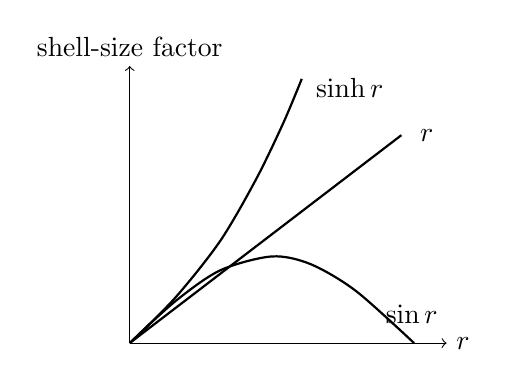
\begin{tikzpicture}[x=1.15cm,y=1.1cm]
\draw[->] (0,0)--(3.5,0) node[right] {$r$};
\draw[->] (0,0)--(0,3.2) node[above] {shell-size factor};

\draw[thick] (0,0)--(3.0,2.4);
\draw (3.1,2.4) node[right] {$r$};

\draw[thick]
plot[smooth] coordinates {(0,0) (0.5,0.48) (1.0,0.84) (1.57,1.0) (2.0,0.91) (2.5,0.60) (3.14,0)};
\draw (2.72,0.55) node[below right] {$\sin r$};

\draw[thick]
plot[smooth] coordinates {(0,0) (0.5,0.52) (1.0,1.18) (1.4,1.90) (1.7,2.55) (1.9,3.05)};
\draw (1.95,2.95) node[right] {$\sinh r$};
\end{tikzpicture}
\caption{The three transverse size factors. The flat, spherical, and hyperbolic cases differ because the shells around us grow respectively like \(r\), \(\sin r\), and \(\sinh r\). The same comparison controls angular size and galaxy counts.}
\end{figure}

The lecture also gives an extrinsic model of hyperbolic space, again strictly as a visualization device. Introduce coordinates \(x\), \(y\), and \(T\), where \(T\) is \emph{not} physical cosmological time, and consider the surface
\begin{equation}
T^2 - x^2 - y^2 = 1.
\end{equation}
This is a hyperboloid. If distances in the embedding space are measured with the Lorentz-signature metric
\begin{equation}
d\ell_{\mathrm{emb}}^2 = dT^2 - dx^2 - dy^2,
\end{equation}
then the hyperboloid is homogeneous. In modern language one says that Lorentz transformations move one point of the hyperboloid to another while preserving the induced geometry. The resulting disk picture is the Poincar\'e disk: far-away objects are squeezed toward the boundary, so they look too small, exactly as the metric calculation says.

\section{Radius of Curvature, Local Flatness, and the Torus Caveat}

Up to now we have mostly discussed \emph{unit} geometries. The unit sphere has radius \(1\), and the unit hyperboloid is normalized similarly. But a real cosmological space comes with a radius of curvature. If that radius is \(a\), then every length is scaled by \(a\), and every squared length is scaled by \(a^2\). That is why the metric of a radius-\(a\) sphere is obtained by multiplying the unit metric by \(a^2\):
\begin{equation}
ds^2 = a^2 d\Omega_n^2.
\end{equation}
Likewise for hyperbolic space,
\begin{equation}
ds^2 = a^2 dh_n^2.
\end{equation}
In explicit radial form one may write
\begin{align}
ds_{\mathrm{sphere}}^2 &= a^2\left(dr^2 + \sin^2 r\, d\Omega_{n-1}^2\right),\\
ds_{\mathrm{hyp}}^2 &= a^2\left(dr^2 + \sinh^2 r\, d\Omega_{n-1}^2\right).
\end{align}
The factor is \(a^2\), not \(a\), because the metric measures squared distance.

This immediately explains local flatness. If \(a\) is very large, then over distances small compared with \(a\), both the sphere and the hyperboloid look almost flat. This is why cosmology can see a geometry that appears extremely flat without thereby proving exact flatness. In the lecture's 2013 observational summary, the data were said to agree with flatness at roughly the percent level, which translates into the statement that any non-flat universe would have to be much larger than the visible region.

A useful rule of thumb is that larger radius means smaller curvature. A basketball looks more curved than the Earth because its radius is smaller. Conversely, a huge sphere looks flatter and flatter locally.

\subsection{Question \& Answer}

Can a universe be flat and still finite?

Yes. This is where the lecture deliberately corrects its earlier simplification. The three simply connected constant-curvature geometries are not the whole story. One can have a flat geometry with nontrivial topology, and the torus is the basic example.

The clean mathematical description of a torus does not begin with a bagel in three-dimensional space. It begins with a flat rectangle whose opposite sides are identified. If one exits through the right edge, one re-enters through the left edge. If one exits through the top, one re-enters through the bottom. The geometry is flat because the local metric is just the flat metric of the rectangle; the nontrivial content is global and topological.

\begin{figure}[htbp]
\centering
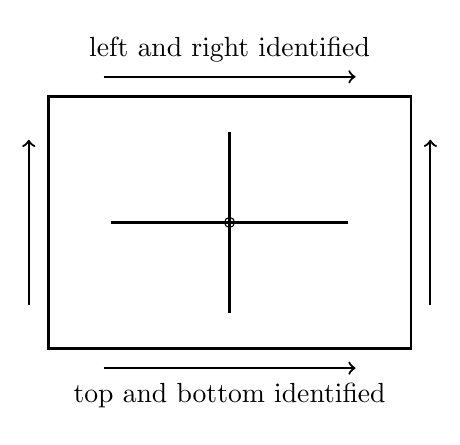
\begin{tikzpicture}[scale=1.0]
\draw[thick] (0,0) rectangle (4.6,3.2);

\draw[->,thick] (0.7,3.45)--(3.9,3.45);
\draw[->,thick] (0.7,-0.25)--(3.9,-0.25);

\draw[->,thick] (-0.25,0.55)--(-0.25,2.65);
\draw[->,thick] (4.85,0.55)--(4.85,2.65);

\draw[thick] (0.8,1.6)--(3.8,1.6);
\draw[thick] (2.3,0.45)--(2.3,2.75);

\draw (2.3,1.6) circle (1.8pt);

\draw (2.3,-0.6) node {top and bottom identified};
\draw (2.3,3.8) node {left and right identified};
\end{tikzpicture}
\caption{A torus described as a rectangle with opposite sides identified. Locally the geometry is flat; globally it is periodic.}
\end{figure}

Such a universe would be observationally equivalent to flat space with periodic copies of everything. If the fundamental cell were small enough, one would see repeated images of the same objects. If it were large enough, one might not notice the periodicity at all. So a universe may indeed be finite and flat, provided the finiteness is topological rather than the result of positive curvature.

\section{From Spatial Geometry to Spacetime Cosmology}

Only after the spatial geometries are understood does the lecture turn back to spacetime. The starting point is Minkowski space, with units chosen so that the speed of light is \(1\):
\begin{equation}
ds^2 = -dt^2 + dx^2 + dy^2 + dz^2.
\end{equation}
The time term comes with the opposite sign from the spatial terms. A light ray is a null ray, meaning that
\begin{equation}
ds^2 = 0.
\end{equation}
If the light ray moves only along the \(x\)-axis, then
\begin{equation}
-dt^2 + dx^2 = 0
\qquad\Rightarrow\qquad
dx = \pm dt.
\end{equation}
So light travels with unit speed to the left or to the right.

Now comes the cosmological substitution. Keep the time piece \(-dt^2\), but replace the flat spatial metric by one of the homogeneous spatial geometries we have just constructed. Then allow the overall size of space to depend on time. To avoid confusion with the earlier fixed radius \(a\), we now write the time-dependent scale factor as \(a(t)\). In compressed form,
\begin{equation}
ds^2 = -dt^2 + a(t)^2 d\Sigma^2,
\end{equation}
where \(d\Sigma^2\) is one of the three spatial metrics:
\begin{align}
d\Sigma^2 &= dx^2 + dy^2 + dz^2 && \text{flat case},\\
d\Sigma^2 &= d\Omega_3^2 && \text{spherical case},\\
d\Sigma^2 &= dh_3^2 && \text{hyperbolic case}.
\end{align}
Thus the three cosmological spacetimes of the lecture are
\begin{align}
ds^2 &= -dt^2 + a(t)^2\left(dx^2+dy^2+dz^2\right),\\
ds^2 &= -dt^2 + a(t)^2 d\Omega_3^2,\\
ds^2 &= -dt^2 + a(t)^2 dh_3^2.
\end{align}

The lecture derives the Hubble law kinematically from this form. Take two points at fixed angular separation \(\theta\) on a sphere of radius \(a(t)\). Their actual distance is
\begin{equation}
D = a(t)\theta.
\end{equation}
Differentiating at fixed \(\theta\),
\begin{equation}
V = \dot a(t)\theta.
\end{equation}
Eliminating \(\theta\) gives
\begin{equation}
V = \frac{\dot a}{a} D.
\end{equation}
So the Hubble parameter is
\begin{equation}
H = \frac{\dot a}{a}.
\end{equation}
Exactly the same kinematics holds in the flat and hyperbolic cases. What matters is not the sign of the spatial curvature, but the fact that all distances are multiplied by the same scale factor.

This is the point at which geometry becomes cosmology proper. Once the metric has been reduced to a single function \(a(t)\), the next question is dynamical: what equations determine \(a(t)\)? The lecture stops here and points forward. Those equations come from general relativity, and in this setting they become the Friedmann equations.

\section{Summary}

The lecture has a very clear arc. First we reopen geometry by dropping flatness while retaining homogeneity. Then we translate geometry into metrics, beginning with flat space and its polar form. Next we build the sphere by replacing the flat shell factor \(r^2\) with \(\sin^2 r\), and we extend the same pattern to the \(3\)-sphere. After that we ask what an astronomer would actually see: in spherical space distant objects look too large and far-away shells contain too few galaxies. Stereographic projection then prepares the eye for hyperbolic space, where the shell factor is \(\sinh^2 r\), distant objects look too small, and the number of objects grows too quickly. Finally we restore the radius of curvature, add the torus as a flat but finite topological exception, and then turn from space to spacetime by inserting the time-dependent scale factor \(a(t)\). At that point the stage is set for the Friedmann dynamics.